\documentclass{standalone}
\usepackage{tikz}
\usetikzlibrary{patterns, positioning}
\usepackage[sfdefault]{ClearSans} %% option 'sfdefault' activates Clear Sans as the default text font
\usepackage[T1]{fontenc}

\begin{document}
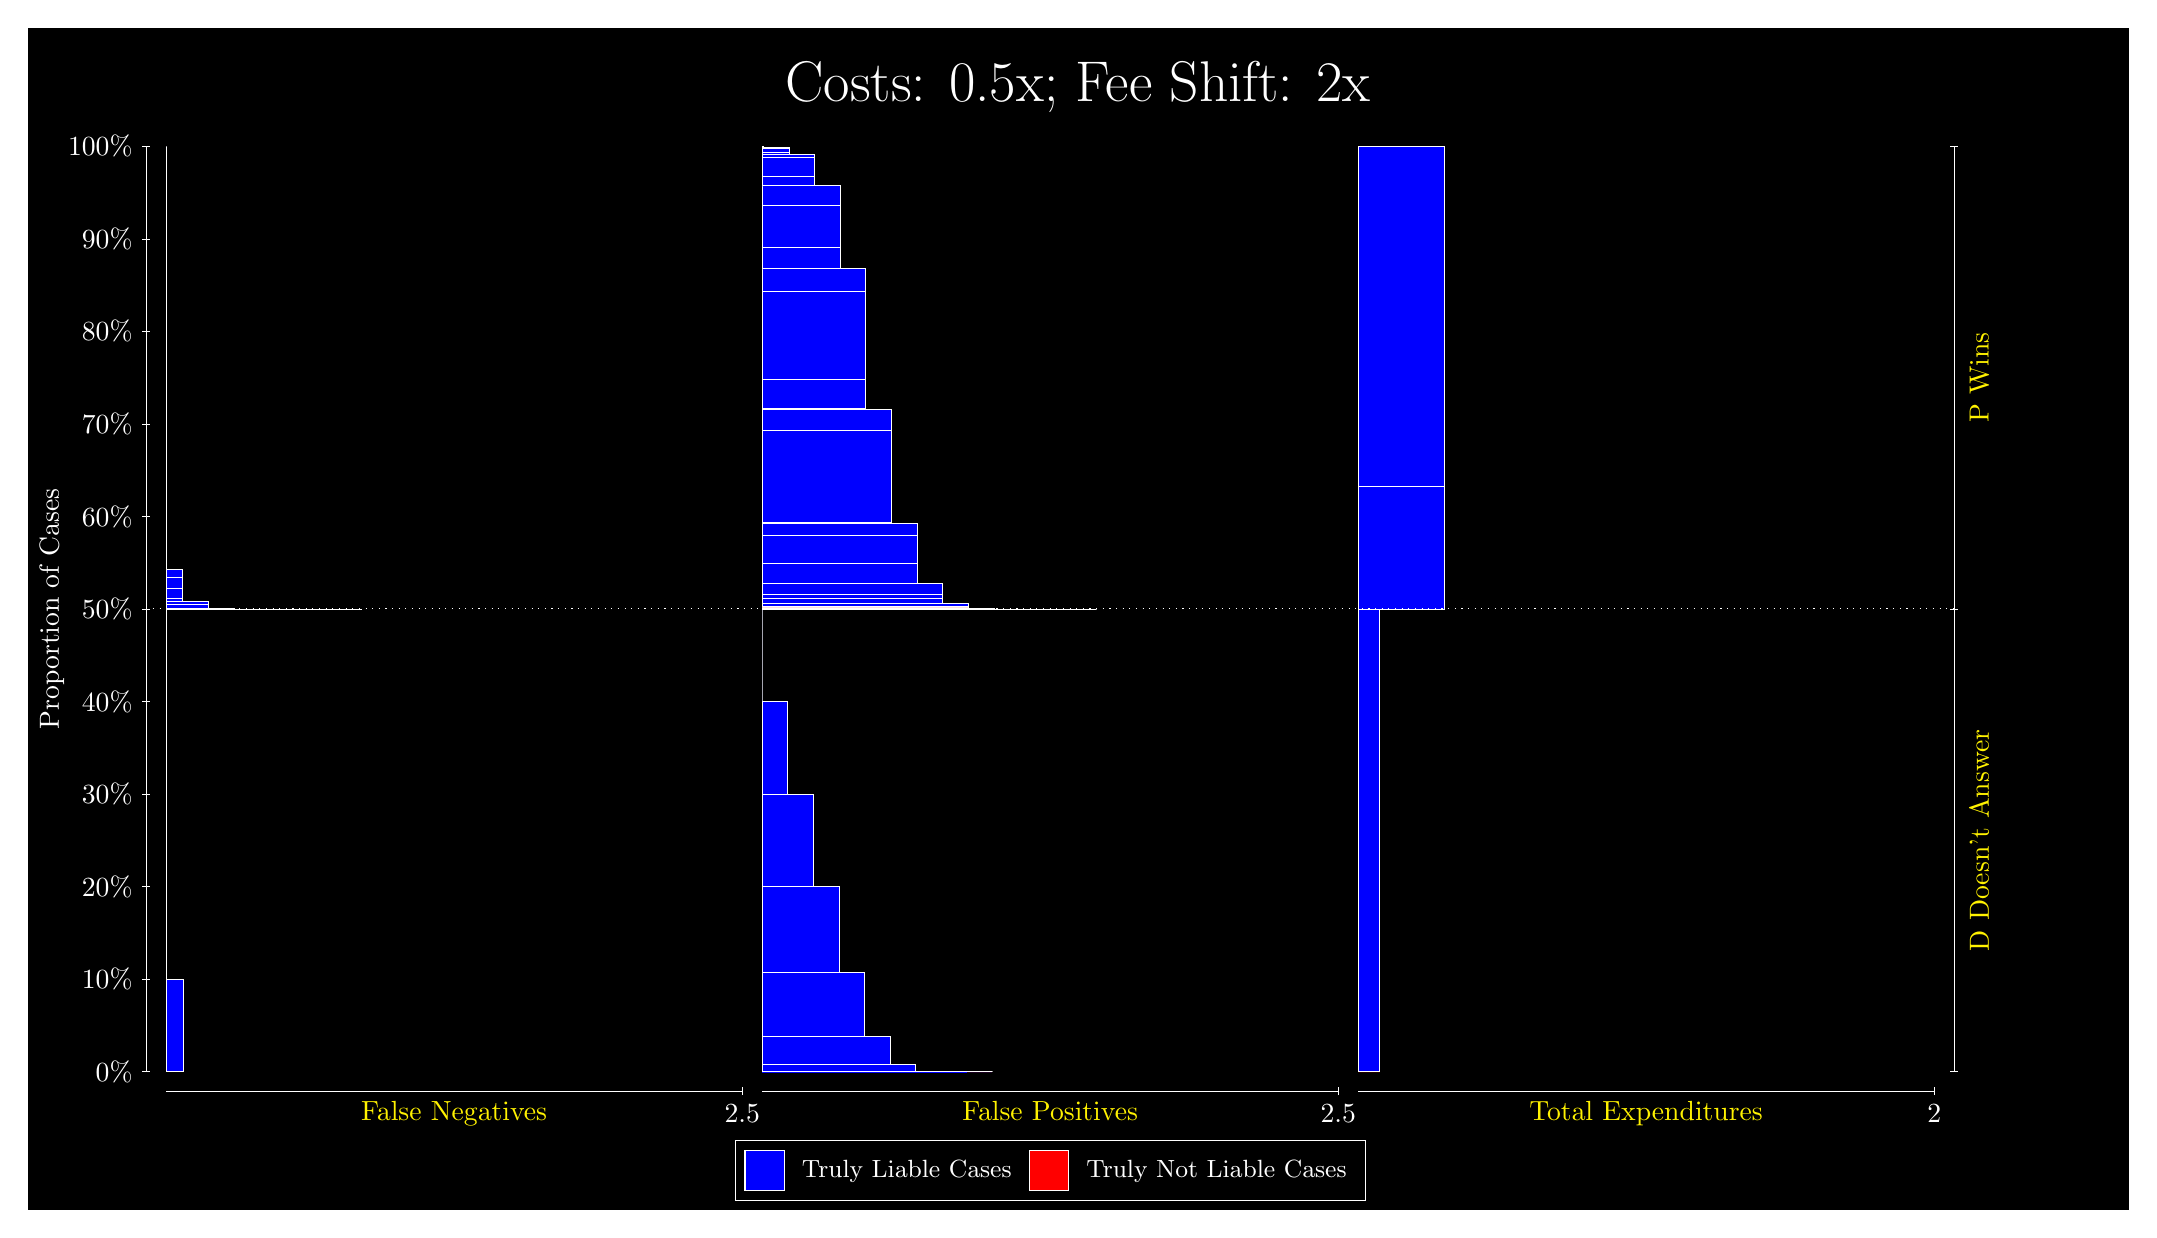
\begin{tikzpicture}
\draw[fill=black] (0,0) rectangle (26.667,15);
\draw[text=white] (0,13.5) rectangle (26.667,15) node[midway] {\huge Costs: 0.5x; Fee Shift: 2x};
\draw[white, very thin] (1.5,1.75) -- (1.5,13.5);
\node[rotate=90, text=white, anchor=center] at (0.3, 7.625) {Proportion of Cases};
\draw[white, very thin] (1.45,1.75) -- (1.55,1.75);
\node[text=white, anchor=east] at (1.45, 1.75) {0\%};
\draw[white, very thin] (1.45,2.925) -- (1.55,2.925);
\node[text=white, anchor=east] at (1.45, 2.925) {10\%};
\draw[white, very thin] (1.45,4.1) -- (1.55,4.1);
\node[text=white, anchor=east] at (1.45, 4.1) {20\%};
\draw[white, very thin] (1.45,5.275) -- (1.55,5.275);
\node[text=white, anchor=east] at (1.45, 5.275) {30\%};
\draw[white, very thin] (1.45,6.45) -- (1.55,6.45);
\node[text=white, anchor=east] at (1.45, 6.45) {40\%};
\draw[white, very thin] (1.45,7.625) -- (1.55,7.625);
\node[text=white, anchor=east] at (1.45, 7.625) {50\%};
\draw[white, very thin] (1.45,8.8) -- (1.55,8.8);
\node[text=white, anchor=east] at (1.45, 8.8) {60\%};
\draw[white, very thin] (1.45,9.975) -- (1.55,9.975);
\node[text=white, anchor=east] at (1.45, 9.975) {70\%};
\draw[white, very thin] (1.45,11.15) -- (1.55,11.15);
\node[text=white, anchor=east] at (1.45, 11.15) {80\%};
\draw[white, very thin] (1.45,12.325) -- (1.55,12.325);
\node[text=white, anchor=east] at (1.45, 12.325) {90\%};
\draw[white, very thin] (1.45,13.5) -- (1.55,13.5);
\node[text=white, anchor=east] at (1.45, 13.5) {100\%};

\draw[white, very thin] (24.457,1.75) -- (24.457,13.5);
\draw[white, very thin] (24.407,1.75) -- (24.507,1.75);
\node[anchor=west] at (24.407, 1.75) {};
\draw[white, very thin] (24.407,7.625) -- (24.507,7.625);
\node[anchor=west] at (24.407, 7.625) {};
\draw[white, very thin] (24.407,13.5) -- (24.507,13.5);
\node[anchor=west] at (24.407, 13.5) {};

\draw[white, very thin, fill=blue] (1.75,1.75) rectangle (1.9696,2.925);
\draw[white, very thin, fill=red] (1.75,2.925) rectangle (1.75,2.925);
\draw[white, very thin, fill=blue] (1.75,2.925) rectangle (1.75,7.625);
\draw[white, very thin, fill=blue] (1.75,7.625) rectangle (4.2384,7.625);
\draw[white, very thin, fill=blue] (1.75,7.625) rectangle (3.9131,7.625);
\draw[white, very thin, fill=blue] (1.75,7.625) rectangle (3.9131,7.625);
\draw[white, very thin, fill=blue] (1.75,7.625) rectangle (3.5878,7.625);
\draw[white, very thin, fill=blue] (1.75,7.625) rectangle (3.2626,7.625);
\draw[white, very thin, fill=blue] (1.75,7.625) rectangle (3.2626,7.625);
\draw[white, very thin, fill=blue] (1.75,7.625) rectangle (2.9373,7.6256);
\draw[white, very thin, fill=blue] (1.75,7.6256) rectangle (2.612,7.6287);
\draw[white, very thin, fill=blue] (1.75,7.6287) rectangle (2.612,7.6363);
\draw[white, very thin, fill=blue] (1.75,7.6363) rectangle (2.2867,7.6843);
\draw[white, very thin, fill=blue] (1.75,7.6843) rectangle (2.2867,7.7263);
\draw[white, very thin, fill=blue] (1.75,7.7263) rectangle (2.2867,7.7264);
\draw[white, very thin, fill=blue] (1.75,7.7264) rectangle (1.9614,7.7666);
\draw[white, very thin, fill=blue] (1.75,7.7666) rectangle (1.9614,7.8894);
\draw[white, very thin, fill=blue] (1.75,7.8894) rectangle (1.9614,8.0253);
\draw[white, very thin, fill=blue] (1.75,8.0253) rectangle (1.9614,8.1252);
\draw[white, very thin, fill=red] (1.75,8.1252) rectangle (1.75,8.1252);
\draw[white, very thin, fill=blue] (1.75,8.1252) rectangle (1.75,13.5);
\draw[white, very thin, fill=red] (9.3189,1.75) rectangle (12.246,1.75);
\draw[white, very thin, fill=blue] (9.3189,1.75) rectangle (12.246,1.75);
\draw[white, very thin, fill=blue] (9.3189,1.75) rectangle (11.921,1.7503);
\draw[white, very thin, fill=blue] (9.3189,1.7503) rectangle (11.596,1.7576);
\draw[white, very thin, fill=blue] (9.3189,1.7576) rectangle (11.271,1.8362);
\draw[white, very thin, fill=blue] (9.3189,1.8362) rectangle (10.945,2.1987);
\draw[white, very thin, fill=blue] (9.3189,2.1987) rectangle (10.62,3.0112);
\draw[white, very thin, fill=blue] (9.3189,3.0112) rectangle (10.295,4.1076);
\draw[white, very thin, fill=blue] (9.3189,4.1076) rectangle (9.9694,5.2753);
\draw[white, very thin, fill=blue] (9.3189,5.2753) rectangle (9.6442,6.45);
\draw[white, very thin, fill=blue] (9.3189,6.45) rectangle (9.3189,7.625);
\draw[white, very thin, fill=red] (9.3189,7.625) rectangle (13.564,7.625);
\draw[white, very thin, fill=blue] (9.3189,7.625) rectangle (13.564,7.625);
\draw[white, very thin, fill=red] (9.3189,7.625) rectangle (13.239,7.625);
\draw[white, very thin, fill=blue] (9.3189,7.625) rectangle (13.239,7.625);
\draw[white, very thin, fill=red] (9.3189,7.625) rectangle (12.913,7.625);
\draw[white, very thin, fill=blue] (9.3189,7.625) rectangle (12.913,7.6251);
\draw[white, very thin, fill=blue] (9.3189,7.6251) rectangle (12.913,7.6251);
\draw[white, very thin, fill=red] (9.3189,7.6251) rectangle (12.588,7.6251);
\draw[white, very thin, fill=blue] (9.3189,7.6251) rectangle (12.588,7.6257);
\draw[white, very thin, fill=red] (9.3189,7.6257) rectangle (12.263,7.6257);
\draw[white, very thin, fill=blue] (9.3189,7.6257) rectangle (12.263,7.6336);
\draw[white, very thin, fill=blue] (9.3189,7.6336) rectangle (11.937,7.6429);
\draw[white, very thin, fill=blue] (9.3189,7.6429) rectangle (11.937,7.6533);
\draw[white, very thin, fill=red] (9.3189,7.6533) rectangle (11.937,7.6533);
\draw[white, very thin, fill=blue] (9.3189,7.6533) rectangle (11.937,7.6909);
\draw[white, very thin, fill=blue] (9.3189,7.6909) rectangle (11.612,7.7638);
\draw[white, very thin, fill=blue] (9.3189,7.7638) rectangle (11.612,7.8134);
\draw[white, very thin, fill=red] (9.3189,7.8134) rectangle (11.612,7.8134);
\draw[white, very thin, fill=blue] (9.3189,7.8134) rectangle (11.612,7.951);
\draw[white, very thin, fill=blue] (9.3189,7.951) rectangle (11.287,8.2042);
\draw[white, very thin, fill=red] (9.3189,8.2042) rectangle (11.287,8.2042);
\draw[white, very thin, fill=blue] (9.3189,8.2042) rectangle (11.287,8.5564);
\draw[white, very thin, fill=blue] (9.3189,8.5564) rectangle (11.287,8.7112);
\draw[white, very thin, fill=blue] (9.3189,8.7112) rectangle (10.962,8.7279);
\draw[white, very thin, fill=red] (9.3189,8.7279) rectangle (10.962,8.7279);
\draw[white, very thin, fill=blue] (9.3189,8.7279) rectangle (10.962,9.8965);
\draw[white, very thin, fill=blue] (9.3189,9.8965) rectangle (10.962,10.157);
\draw[white, very thin, fill=blue] (9.3189,10.157) rectangle (10.636,10.179);
\draw[white, very thin, fill=blue] (9.3189,10.179) rectangle (10.636,10.544);
\draw[white, very thin, fill=red] (9.3189,10.544) rectangle (10.636,10.544);
\draw[white, very thin, fill=blue] (9.3189,10.544) rectangle (10.636,11.658);
\draw[white, very thin, fill=blue] (9.3189,11.658) rectangle (10.636,11.947);
\draw[white, very thin, fill=blue] (9.3189,11.947) rectangle (10.311,11.947);
\draw[white, very thin, fill=blue] (9.3189,11.947) rectangle (10.311,12.224);
\draw[white, very thin, fill=blue] (9.3189,12.224) rectangle (10.311,12.752);
\draw[white, very thin, fill=blue] (9.3189,12.752) rectangle (10.311,13);
\draw[white, very thin, fill=blue] (9.3189,13) rectangle (9.9857,13);
\draw[white, very thin, fill=blue] (9.3189,13) rectangle (9.9857,13.123);
\draw[white, very thin, fill=blue] (9.3189,13.123) rectangle (9.9857,13.358);
\draw[white, very thin, fill=blue] (9.3189,13.358) rectangle (9.9857,13.399);
\draw[white, very thin, fill=blue] (9.3189,13.399) rectangle (9.6604,13.43);
\draw[white, very thin, fill=blue] (9.3189,13.43) rectangle (9.6604,13.472);
\draw[white, very thin, fill=blue] (9.3189,13.472) rectangle (9.6604,13.489);
\draw[white, very thin, fill=blue] (9.3189,13.489) rectangle (9.3351,13.499);
\draw[white, very thin, fill=blue] (9.3189,13.499) rectangle (9.3351,13.499);
\draw[white, very thin, fill=blue] (9.3189,13.499) rectangle (9.3189,13.5);
\draw[white, very thin, fill=red] (16.888,1.75) rectangle (17.162,1.75);
\draw[white, very thin, fill=blue] (16.888,1.75) rectangle (17.162,7.625);
\draw[white, very thin, fill=red] (16.888,7.625) rectangle (17.986,7.625);
\draw[white, very thin, fill=blue] (16.888,7.625) rectangle (17.986,9.183);
\draw[white, very thin, fill=red] (16.888,9.183) rectangle (17.986,9.183);
\draw[white, very thin, fill=blue] (16.888,9.183) rectangle (17.986,13.5);
\draw[white, dotted] (1.5,7.625) -- (24.457,7.625);
\draw[white, very thin] (1.75,1.5) -- (9.0689,1.5);
\node[text=yellow, anchor=north] at (5.4094, 1.5) {False Negatives};
\draw[white, very thin] (9.0689,1.45) -- (9.0689,1.55);
\node[text=white, anchor=north] at (9.0689, 1.45) {2.5};

\draw[white, very thin] (9.3189,1.5) -- (16.638,1.5);
\node[text=yellow, anchor=north] at (12.978, 1.5) {False Positives};
\draw[white, very thin] (16.638,1.45) -- (16.638,1.55);
\node[text=white, anchor=north] at (16.638, 1.45) {2.5};

\draw[white, very thin] (16.888,1.5) -- (24.207,1.5);
\node[text=yellow, anchor=north] at (20.547, 1.5) {Total Expenditures};
\draw[white, very thin] (24.207,1.45) -- (24.207,1.55);
\node[text=white, anchor=north] at (24.207, 1.45) {2};

\node[text=yellow, centered, rotate=90] at (24.777, 4.6875) {D Doesn't Answer};
\node[text=yellow, centered, rotate=90] at (24.777, 10.563) {P Wins};

\draw (12.978300999999998,1.5) node[draw=none] (baseCoordinate) {};
\begin{scope}[align=center]
        \matrix[scale=0.5, draw=white, below=0.5cm of baseCoordinate, nodes={draw}, column sep=0.1cm]{
            \node[rectangle, draw, minimum width=0.5cm, minimum height=0.5cm, fill=blue] {}; &
            \node[draw=none, font=\small, text=white] (B) {Truly Liable Cases}; &
            \node[rectangle, draw, minimum width=0.5cm, minimum height=0.5cm, fill=red] {}; &
            \node[draw=none, font=\small, text=white] (B) {Truly Not Liable Cases}; \\
            };
\end{scope}

\end{tikzpicture}
\end{document}